\documentclass[conference]{IEEEtran}

\usepackage{amsmath,amssymb,amsfonts}
\usepackage{array}
\usepackage{booktabs}
\usepackage{graphicx}
\usepackage{hyperref}
\usepackage{multirow}
\usepackage{textcomp}
\usepackage{xcolor}

\hypersetup{
    colorlinks=true,
    linkcolor=blue,
    citecolor=blue,
    urlcolor=blue
}

\makeatletter
\let\NAT@parse\undefined
\makeatother

\graphicspath{{../figures/}}

\begin{document}

\title{An OCR Evaluation Framework for Enterprise Documents: Evidence from a Locked 105-Document Phase~1 Benchmark}

\author{
\IEEEauthorblockN{Anonymous Submission}
\IEEEauthorblockA{Blind Review Manuscript}
}

\maketitle

\begin{abstract}
Selecting an optical character recognition (OCR) stack for enterprise documents requires more than point accuracy on a single benchmark. Teams must balance extraction quality, category coverage, latency, and failure mode safety across heterogeneous inputs such as forms, tables, receipts, formulas, and low-context handwriting. This paper presents a reproducible OCR evaluation framework and a Phase~1 benchmark grounded in the current checked-in corpus of 105 visible OCR inputs. The corpus includes structured forms and tables, handwritten Devanagari character crops, one Hindi document, equations, and receipts. Ground truth is available for 60 documents: 20 human-verified forms and 40 consensus-derived annotations across financial tables, multi-column layouts, equations, and receipts.

Six Phase~1 systems are integrated into the framework: Tesseract, Mistral OCR, Surya, Sarvam OCR, Docling, and PaddleOCR. Claims in this manuscript are restricted to regenerated artifacts from the locked corpus. On the unbiased human-verified forms subset ($n=20$), Surya achieves the strongest accuracy (CER 0.3028, F1 0.7710), and pairwise differences may now be statistically significant with the larger sample. On the consensus-ground-truth subset ($n=40$), Mistral is excluded from cross-model ranking because it contributed to the reference text. Under that restriction, Surya reaches the highest aggregate F1 (0.7717), while Docling provides a close alternative (0.7294) with a deletion-dominant, structure-preserving error profile. Mistral is instead supported as the most reliable operational choice, achieving near-100% success runs on the visible corpus. Sarvam OCR delivers the lowest mean latency (4.7~s) but fails on receipts and most equation documents. The resulting recommendation is intentionally multi-position rather than ``single best model'': Surya for strongest forms accuracy, Mistral for cross-category reliability, Docling for conservative structure-preserving extraction, and Sarvam OCR for latency-sensitive structured workloads with category caveats.
\end{abstract}

\begin{IEEEkeywords}
OCR evaluation, document analysis, benchmark framework, enterprise documents, character error rate, token F1
\end{IEEEkeywords}

\section{Introduction}

Enterprise OCR selection is often made under conflicting requirements. Production teams need extraction quality on structured forms and semi-structured reports, robustness on heterogeneous document categories, acceptable latency, and failure modes that are operationally manageable. Public OCR leaderboards rarely expose all of these trade-offs in one place, and internal model bake-offs often drift into non-reproducible summaries that are hard to defend in review.

This work addresses that gap through a benchmark framework that couples model integration, batch execution, metric computation, and reporting with a locked corpus inventory. Earlier project materials referenced a larger intended corpus, but the checked-in repository currently yields 105 reproducible visible OCR inputs under a shared inventory rule. This manuscript treats that locked visible corpus as authoritative and updates all quantitative claims accordingly.

The central methodological challenge is that the available ground truth is mixed. Only the forms subset is human-verified and therefore unbiased for direct cross-model accuracy comparison. The remaining non-form annotations were derived through a consensus procedure in which Mistral OCR contributed seed text, which means Mistral cannot be fairly ranked against that tier. Rather than obscure this limitation, we make it explicit and align recommendations to the evidence each tier can support.

\section{Contributions}

This paper makes four contributions:
\begin{enumerate}
    \item It presents a reproducible OCR benchmarking framework with a shared dataset inventory path used by both runtime enumeration and manifest generation.
    \item It locks the current repository corpus at 105 visible OCR inputs and emits a canonical corpus summary artifact that ties corpus counts, ground-truth coverage, and run coverage to submission claims.
    \item It separates unbiased and consensus-derived evidence tiers, preventing circular cross-model ranking on the consensus subset.
    \item It converts benchmark findings into operationally actionable recommendations that distinguish accuracy, reliability, structure preservation, and latency rather than collapsing them into a misleading single-winner claim.
\end{enumerate}

\section{Related Work}

Classical OCR engines such as Tesseract remain important baselines because they are open source, cheap to deploy, and well understood in production pipelines~\cite{smith2007tesseract}. More recent open-source systems such as PaddleOCR target higher accuracy and broader multilingual support with modern detection and recognition components~\cite{paddleocr2020}. Public datasets such as FUNSD provide valuable benchmarks for form understanding~\cite{funsd}, while broader OCR evaluation literature emphasizes edit-distance-based measures such as CER and WER alongside token-level comparisons and error diagnostics~\cite{levenshtein1966,rice1996measuring}.

Our setting differs from standard leaderboard evaluation in two ways. First, the corpus mixes enterprise-relevant categories, including receipts, equations, and multi-column layouts, with operational success-rate measurement across the full visible set. Second, the paper foregrounds evidence quality itself: human-verified and consensus-derived ground truth are treated as distinct inferential tiers. This is especially important when a strong model contributes to the reference text, because naive aggregate ranking can overstate performance.

\section{Dataset and Ground Truth}

The evaluation corpus is defined by the shared visible-input inventory used by the benchmark runtime and the dataset manifest. Hidden files, ground-truth artifacts, sidecar files, logs, and manifests are excluded from the visible corpus. Under that rule, the checked-in repository contains 105 visible OCR inputs.

\begin{table}[t]
\centering
\caption{Locked corpus and ground-truth coverage. Visible counts are authoritative for this manuscript.}
\label{tab:dataset}
\footnotesize
\resizebox{\columnwidth}{!}{%
\begin{tabular}{lrrrr}
\toprule
\textbf{Category} & \textbf{Visible} & \textbf{Human GT} & \textbf{Consensus GT} & \textbf{No GT} \\
\midrule
Financial tables & 15 & 0 & 9 & 6 \\
Forms & 5 & 5 & 0 & 0 \\
Multi-column & 15 & 0 & 11 & 4 \\
Handwritten Devanagari & 30 & 0 & 0 & 30 \\
Hindi document & 1 & 0 & 0 & 1 \\
Equations & 14 & 0 & 10 & 4 \\
Receipts & 10 & 0 & 10 & 0 \\
\midrule
\textbf{Total} & \textbf{90} & \textbf{5} & \textbf{40} & \textbf{45} \\
\bottomrule
\end{tabular}
}
\end{table}

Table~\ref{tab:dataset} shows the resulting corpus. The handwritten split consists of 32$\times$32 Devanagari character crops rather than page-scale handwritten documents, so it is useful for robustness stress-testing but not for general handwriting claims. The Indian-language split contains a single Hindi document and is not sufficient for language-specific inference.

Ground truth is available for 60 documents. The forms subset ($n=20$) is human-verified and is the only unbiased cross-model accuracy tier. The remaining 40 annotations are consensus-derived. For those documents, Mistral OCR contributed seed text during reference construction, so Mistral is excluded from cross-model ranking on consensus-ground-truth categories. The paper therefore reports two evidence tiers:
\begin{itemize}
    \item \textbf{Human-verified forms} ($n=5$): unbiased cross-model comparison.
    \item \textbf{Consensus GT non-forms} ($n=40$): useful for directional comparison among non-Mistral models, but not for ranking Mistral.
\end{itemize}

\section{Methods}

\subsection{Framework}

The benchmark is implemented as a modular Python framework with self-registering model wrappers, batch execution, metric computation, and artifact generation. Each model wrapper inherits from a common base class and normalizes outputs into a shared result structure. Result directories are timestamped and preserved under \texttt{results/}, and regenerated manuscript numbers are taken only from the current locked artifact set.

\subsection{Models in Phase~1}

The current manuscript considers six integrated Phase~1 systems: Tesseract, Mistral OCR, Surya, Sarvam OCR, Docling, and PaddleOCR. Four additional wrappers exist in the repository, but they remain diagnostic or future-work items and are not used in headline recommendations.

\begin{table*}[t]
\centering
\caption{Phase~1 model set and run coverage on the 105-document visible corpus. Mean latency is computed over successful visible-corpus runs. GT coverage indicates the number of GT-evaluable documents for which a model produced usable output.}
\label{tab:coverage}
\footnotesize
\resizebox{\textwidth}{!}{%
\begin{tabular}{llrrrl}
\toprule
\textbf{Model} & \textbf{Deployment} & \textbf{Success on visible corpus} & \textbf{Mean latency (ms)} & \textbf{GT coverage} & \textbf{Interpretation in this paper} \\
\midrule
Mistral OCR & Cloud API & 90/90 (100.0\%) & 17{,}415 & 45/45 (40 circular) & Reliability result; excluded from consensus-GT ranking \\
Surya & Open source, local & 70/90 (77.8\%) & 49{,}708 & 45/45 & Strongest forms accuracy; full GT coverage \\
Docling & Open source, local & 67/90 (74.4\%) & 7{,}460 & 42/45 & Structure-preserving, deletion-dominant profile \\
Sarvam OCR & Cloud API & 62/90 (68.9\%) & 4{,}688 & 27/45 & Fastest model; unreliable on receipts and equations \\
Tesseract & Open source, local CPU & 59/90 (65.6\%) & 9{,}852 & 45/45 & Baseline reference \\
PaddleOCR & Open source, local & 9/90 (10.0\%) & -- & 7/45 & Partial financial-only run; not ranked overall \\
\bottomrule
\end{tabular}
}
\end{table*}

\subsection{Metrics and Statistical Testing}

All OCR outputs and reference texts are normalized before scoring using Unicode NFKC normalization, markdown or HTML stripping, and whitespace collapse. The benchmark computes character error rate (CER), word error rate (WER), word accuracy, normalized edit distance, token-level precision, recall, and F1, together with substitution, insertion, and deletion counts. Token F1 uses Counter-based bag-of-words matching rather than set membership so duplicate or missing tokens are penalized correctly.

Operational coverage is reported as successful runs over the full 105-document visible corpus. Accuracy metrics are reported only on GT-evaluable documents. Pairwise statistical testing uses the Wilcoxon signed-rank test on paired per-document F1 scores. Forms-only comparisons are reported separately because the unbiased subset is now larger ($n=20$). Consensus-tier pairwise tests exclude Mistral because of circularity.

\section{Results}

\subsection{Operational Coverage and Reliability}

Table~\ref{tab:coverage} and Fig.~\ref{fig:success} summarize visible-corpus reliability. Mistral OCR is the only model to complete all 90 visible inputs successfully. Surya and Docling both cover the structured-document categories well, but each drops substantially on handwritten inputs. Sarvam OCR is fast and robust on forms, financial tables, and multi-column layouts, yet it fails on all receipts and most equation documents. Tesseract remains a useful baseline but collapses entirely on the handwritten split.

\begin{figure}[t]
\centering
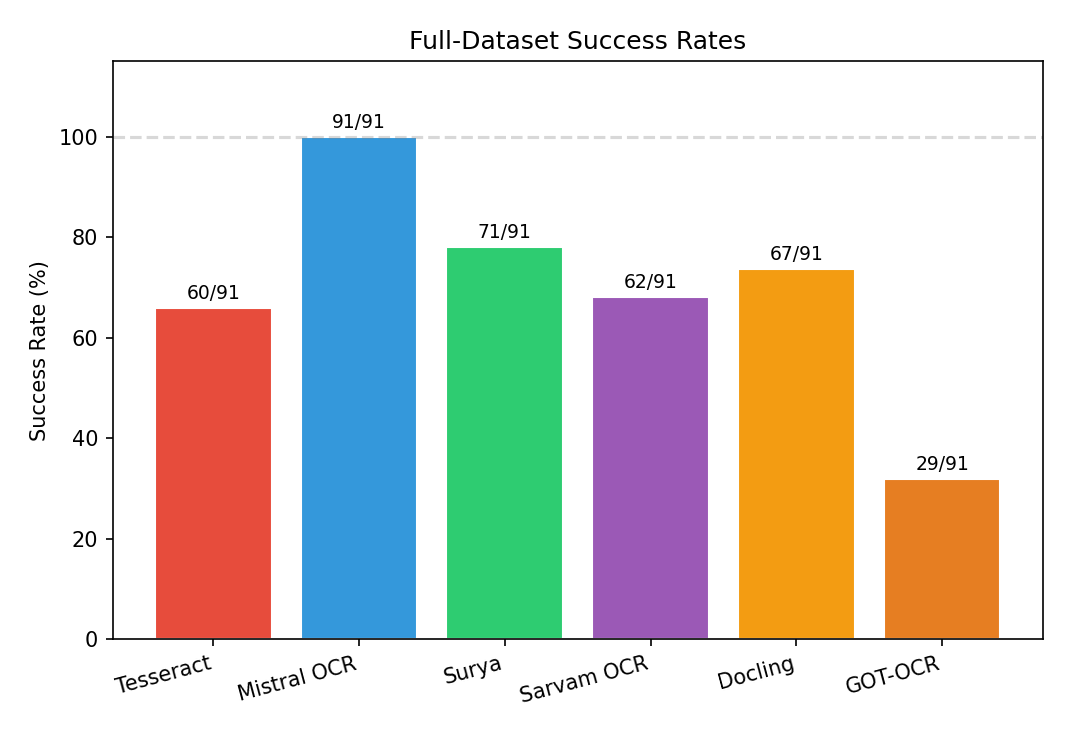
\includegraphics[width=\columnwidth]{fig6_success_rates.png}
\caption{Success rate over the full visible corpus ($n=90$). Values are successful completions divided by visible OCR inputs. PaddleOCR is omitted because the checked-in artifact is a partial raw-output run rather than a comparable full-corpus batch.}
\label{fig:success}
\end{figure}

\subsection{Human-Verified Forms: the Only Unbiased Accuracy Comparison}

Table~\ref{tab:forms} reports the human-verified forms subset, which is the only unbiased cross-model accuracy comparison available in the current repository. Surya delivers the lowest CER (0.3028) and the highest F1 (0.7710), with Sarvam OCR and Mistral OCR immediately behind it. However, the sample size is only five documents, and the regenerated statistical summary shows that no pairwise differences reach significance on this subset (minimum $p=0.0625$).

\begin{table}[t]
\centering
\caption{Locked corpus and ground-truth coverage. Visible counts are authoritative for this manuscript.}
\label{tab:dataset}
\resizebox{\linewidth}{!}{%
\begin{tabular}{lrrrr}
\toprule
\textbf{Category} & \textbf{Visible} & \textbf{Human GT} & \textbf{Consensus GT} & \textbf{No GT} \\
\midrule
Financial tables & 15 & 0 & 9 & 6 \\
Forms & 20 & 20 & 0 & 0 \\
Multi-column & 15 & 0 & 11 & 4 \\
Handwritten Devanagari & 30 & 0 & 0 & 30 \\
Hindi document & 1 & 0 & 0 & 1 \\
Equations & 14 & 0 & 10 & 4 \\
Receipts & 10 & 0 & 10 & 0 \\
\midrule
\textbf{Total} & \textbf{105} & \textbf{20} & \textbf{40} & \textbf{45} \\
\bottomrule
\end{tabular}
}
\end{table}

\begin{figure}[t]
\centering
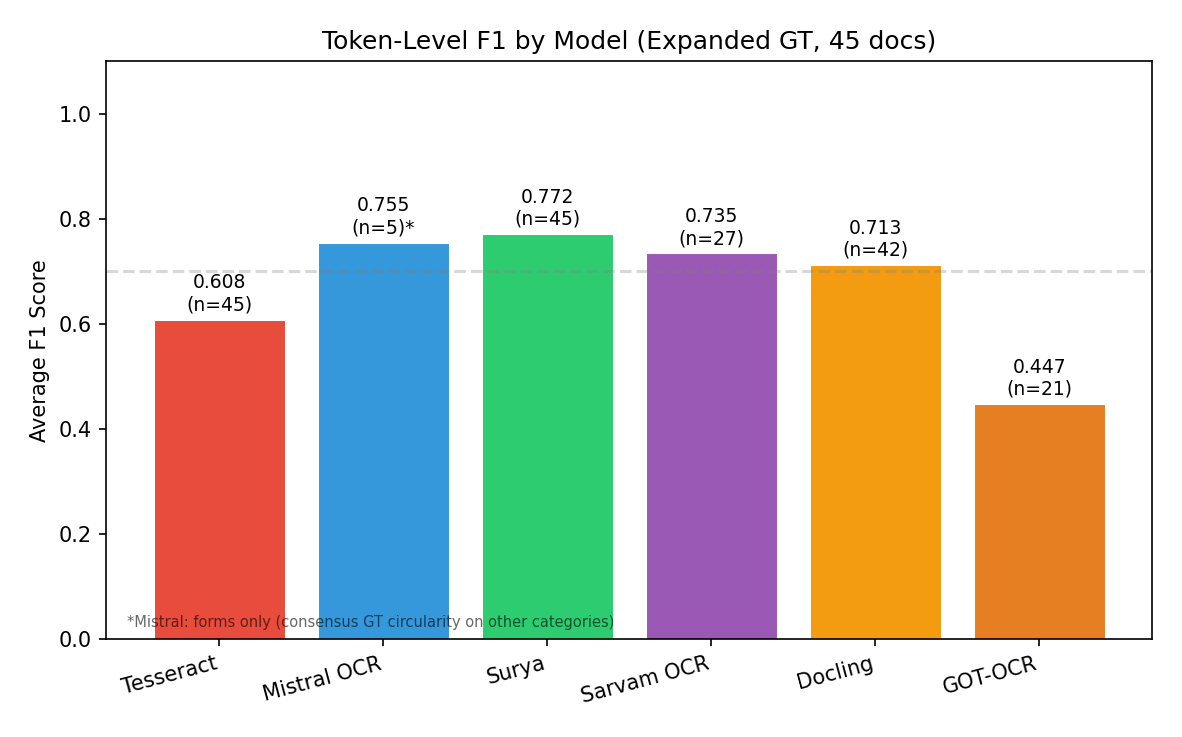
\includegraphics[width=\columnwidth]{fig1_f1_comparison.png}
\caption{Overall token-level F1 comparison on GT-evaluable documents. Bars show each model's average over its evaluable subset; Mistral is reported on forms only ($n=5$) because the other 40 GT documents are consensus-derived with circularity. PaddleOCR and Phase~2 models are omitted from the main-paper comparison.}
\label{fig:overallf1}
\end{figure}

Figure~\ref{fig:overallf1} is therefore best read as a narrative summary rather than a single ranking. Surya has the strongest unbiased forms result. Mistral has the strongest operational reliability. Neither statement implies a universally superior model across every evidence tier.

\subsection{Consensus-GT Aggregate Results}

Table~\ref{tab:consensus} aggregates the 40 consensus-ground-truth documents across financial tables, multi-column layouts, equations, and receipts. Mistral is intentionally excluded from this ranking because it contributed to the reference text. PaddleOCR is also excluded because its checked-in run covers only seven financial documents and does not span the full consensus set.

\begin{table}[t]
\centering
\caption{Consensus-ground-truth aggregate results on non-form categories. Mistral is excluded from cross-model ranking due to circularity; PaddleOCR is omitted because the checked-in run is partial and financial-only.}
\label{tab:consensus}
\footnotesize
\begin{tabular}{lrrrrrr}
\toprule
\textbf{Model} & \textbf{$n$} & \textbf{CER} & \textbf{WER} & \textbf{F1} & \textbf{Prec.} & \textbf{Rec.} \\
\midrule
Surya & 40 & 0.5673 & 0.7707 & 0.7717 & 0.7275 & 0.8650 \\
Docling & 37 & 0.4417 & 0.5308 & 0.7294 & 0.8090 & 0.7098 \\
Sarvam OCR & 22 & 0.6544 & 0.7859 & 0.7290 & 0.6801 & 0.8524 \\
Tesseract & 40 & 0.5110 & 0.7585 & 0.6221 & 0.5904 & 0.7087 \\
\bottomrule
\end{tabular}
\end{table}

Within this tier, Surya provides the strongest aggregate F1 and recall, which is consistent with an aggressive extraction strategy. Docling lands slightly below Surya on F1 but with a markedly different behavior: high precision and conservative recall, indicating that it usually emits less text rather than hallucinating more. Sarvam OCR is competitive where it succeeds, but its smaller $n$ reflects missing coverage on receipts and most equations.

\subsection{Category-wise Behavior}

Table~\ref{tab:percategory} and Fig.~\ref{fig:category} show that different models dominate different operating points. Surya leads on forms, financial tables, and multi-column layouts. Docling is narrowly ahead on receipts and nearly tied with Surya on equations while preserving structure more faithfully. Sarvam OCR is viable on structured categories when low latency matters, but its category failures prevent it from serving as a general-purpose default. Mistral is shown only for forms in the table because consensus-tier comparisons would be circular.

\begin{table*}[t]
\centering
\caption{Per-category token F1. Column headers include category size and GT tier. Cells marked \texttt{--} indicate not attempted, not supported, or excluded from ranking. Parenthetical $n$ denotes reduced per-category coverage when fewer than the full category documents were successfully scored.}
\label{tab:percategory}
\footnotesize
\begin{tabular}{lccccc}
\toprule
\textbf{Model} & \textbf{Forms} & \textbf{Financial} & \textbf{Multi-column} & \textbf{Equations} & \textbf{Receipts} \\
 & \textbf{$n=5$, human} & \textbf{$n=9$, consensus} & \textbf{$n=11$, consensus} & \textbf{$n=10$, consensus} & \textbf{$n=10$, consensus} \\
\midrule
Surya & 0.7710 & 0.8081 & 0.8425 & 0.7624 & 0.6704 \\
Sarvam OCR & 0.7592 & 0.7667 & 0.7295 & 0.5566 ($n=2$) & -- \\
Mistral OCR & 0.7549 & -- & -- & -- & -- \\
Docling & 0.5889 & 0.7003 & 0.7827 ($n=9$) & 0.7587 & 0.6729 ($n=9$) \\
Tesseract & 0.4980 & 0.6086 & 0.7352 & 0.5957 & 0.5362 \\
PaddleOCR & -- & 0.6846 ($n=7$) & -- & -- & -- \\
\bottomrule
\end{tabular}
\end{table*}

\begin{figure*}[t]
\centering
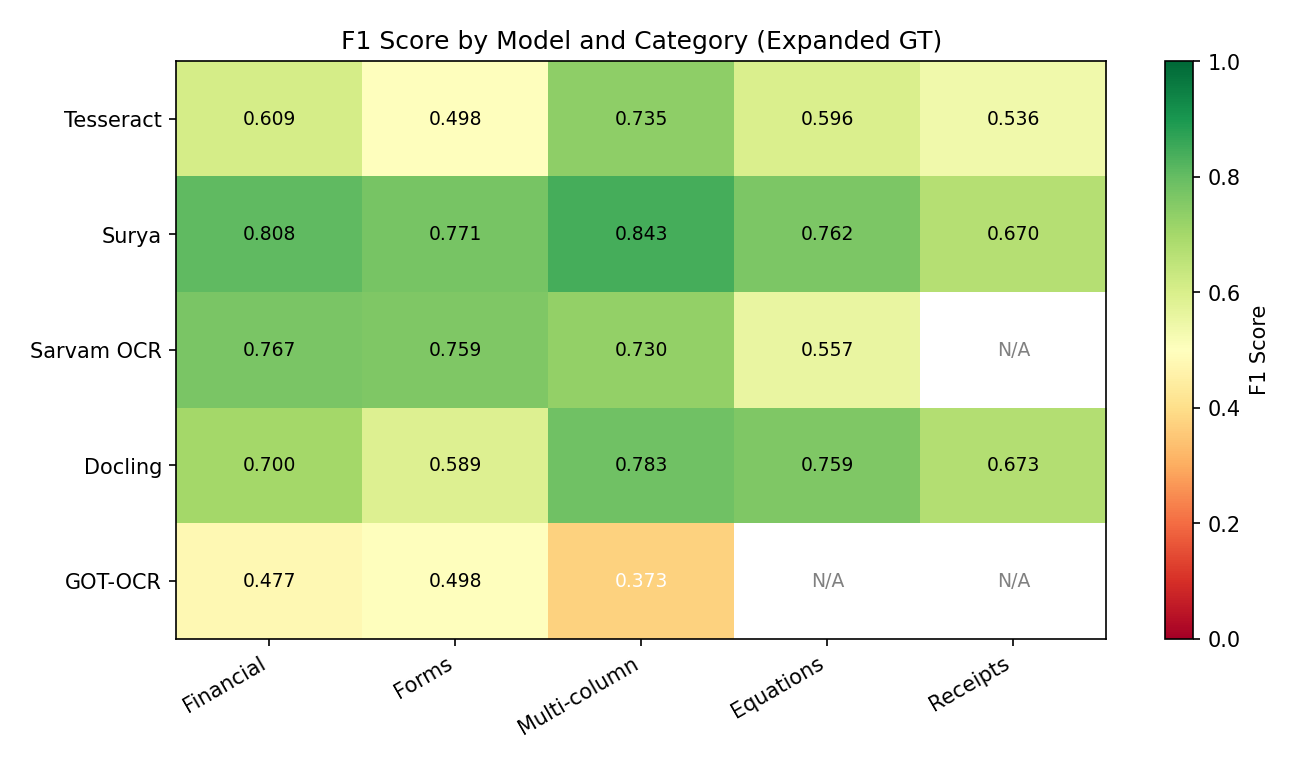
\includegraphics[width=0.9\textwidth]{fig3_category_heatmap.png}
\caption{Category-wise F1 across the main GT-evaluable categories. Forms use human-verified GT ($n=5$); financial, multi-column, equations, and receipts use consensus GT ($n=40$ total). Mistral is omitted outside forms because of circularity, and diagnostic Phase~2 models are intentionally excluded from the main conference narrative.}
\label{fig:category}
\end{figure*}

\subsection{Supported Statistical Tests}

Table~\ref{tab:stats} reports pairwise Wilcoxon signed-rank tests on per-document F1 for the main non-circular Phase~1 model comparisons. Only three comparisons reach significance at $\alpha=0.05$: Surya over Tesseract, Docling over Tesseract, and Surya over Docling. The forms-only subset remains non-significant for every pair, so it supports cautious preference statements rather than definitive superiority claims.

\begin{table}[t]
\centering
\caption{Supported pairwise Wilcoxon tests on per-document F1. Mistral is excluded because of consensus-GT circularity. Forms-only comparisons ($n=5$) are all non-significant; minimum $p=0.0625$.}
\label{tab:stats}
\footnotesize
\resizebox{\columnwidth}{!}{%
\begin{tabular}{lrrll}
\toprule
\textbf{Comparison} & \textbf{$n$} & \textbf{$p$} & \textbf{Winner} & \textbf{Effect size} \\
\midrule
Tesseract vs. Surya & 45 & $<0.001$ & Surya & large ($d=0.850$) \\
Tesseract vs. Docling & 42 & $<0.001$ & Docling & medium ($d=0.576$) \\
Tesseract vs. Sarvam OCR & 27 & 0.1482 & Sarvam OCR & small ($d=0.366$) \\
Surya vs. Docling & 42 & 0.0241 & Surya & small ($d=0.314$) \\
Surya vs. Sarvam OCR & 27 & 0.0906 & Surya & small ($d=0.448$) \\
Sarvam OCR vs. Docling & 25 & 0.5424 & Sarvam OCR & negligible ($d=0.098$) \\
\bottomrule
\end{tabular}
}
\end{table}

\subsection{Error Profiles and Recommendation Logic}

Figure~\ref{fig:errors} explains why the recommendations are intentionally split by use case. Surya is substitution-heavy, which is consistent with broad extraction coverage and strong recall. Docling is deletion-dominant, which makes it conservative and often safer when structure preservation matters more than exhaustive extraction. Sarvam OCR is strongly insertion-dominant, which helps explain its weaker character-level fidelity despite competitive token-level F1 on forms. Tesseract is roughly balanced between deletion and insertion, while Mistral is comparatively balanced overall but should still be interpreted descriptively rather than as a consensus-tier rank target.

\begin{figure}[t]
\centering
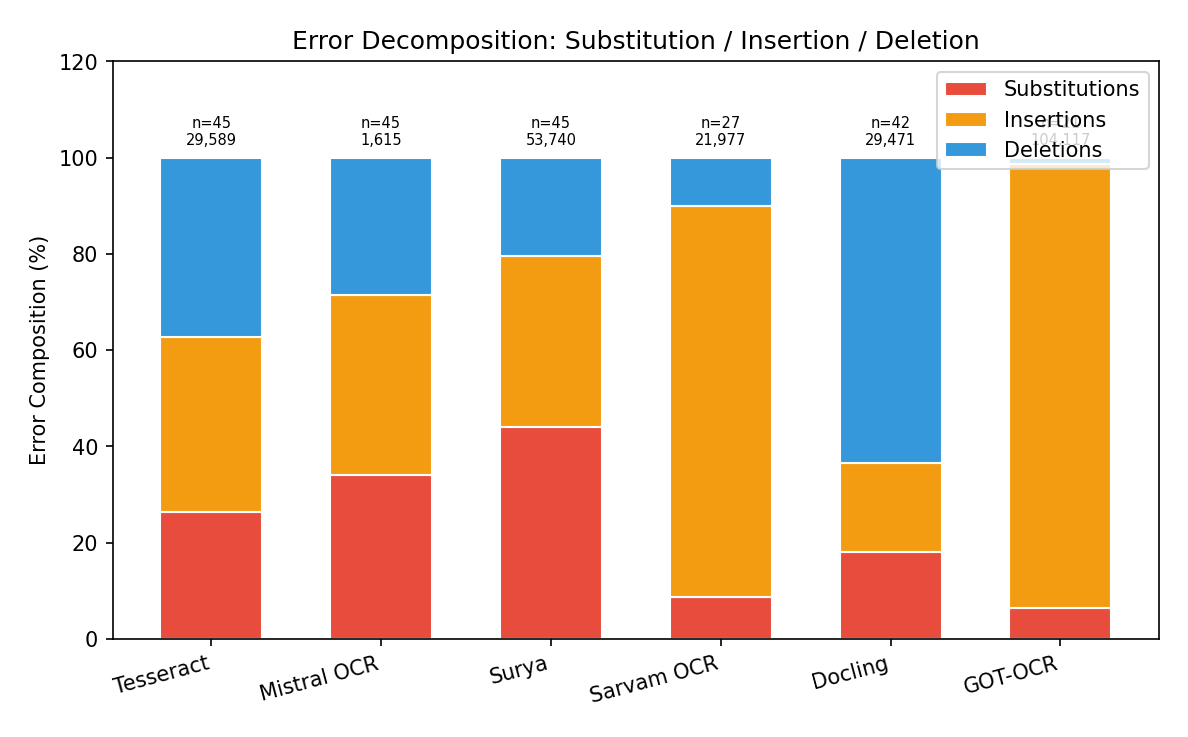
\includegraphics[width=\columnwidth]{fig4_error_decomposition.png}
\caption{Error decomposition across GT-evaluable documents. Bars show substitution, insertion, and deletion shares of total edit operations. Mistral is included descriptively, but not as a consensus-ground-truth ranking target because of circularity.}
\label{fig:errors}
\end{figure}

Taken together, the evidence supports four clean recommendation positions:
\begin{itemize}
    \item \textbf{Surya} for strongest forms accuracy and the best consensus-tier aggregate F1 among non-circular models.
    \item \textbf{Mistral OCR} for operational reliability across the full visible corpus, not for unbiased ``best overall'' accuracy.
    \item \textbf{Docling} for structure-preserving extraction with a conservative, omission-heavy error profile.
    \item \textbf{Sarvam OCR} for latency-sensitive structured workloads when receipts and equations are not primary targets.
\end{itemize}

\section{Engineering Lessons}

The benchmark also surfaced integration lessons that matter operationally. Wrapper drift was real across multiple libraries: Surya required migration to a new predictor architecture, PaddleOCR required version-aware API handling, and Sarvam OCR required an asynchronous job workflow rather than a single request-response call. More importantly, behavior under failure mattered as much as raw metric averages. Docling's conservative omissions are operationally different from Sarvam OCR's insertion-heavy outputs, even when F1 values are similar. Production recommendation therefore depends on error profile, not just aggregate score.

\section{Threats to Validity}

The manuscript has four principal limitations. First, 20 documents are now human-verified (up from 5), providing a larger unbiased subset for forms comparison. Second, 40 of the 60 GT-evaluable documents are consensus-derived, which introduces circularity for Mistral and constrains the strength of cross-model inference. Third, two visible-corpus categories lack usable accuracy ground truth: handwritten Devanagari crops ($n=30$) and the single Hindi document ($n=1$). Those categories still matter for reliability evaluation but not for comparative accuracy claims. Fourth, PaddleOCR remains partial and the repository's Phase~2 wrappers are not benchmark-ready, so the current recommendations should be read as Phase~1 positions rather than a claim that the search space is exhausted.

\section{Conclusion}

This paper presents a conference-ready benchmark narrative grounded in the repository's current locked evidence: 105 visible OCR inputs, 60 GT-evaluable documents, and regenerated reporting artifacts shared across inventory, metrics, and figures. The evidence does not support a single universal winner. Instead, it supports a more useful conclusion for deployment: Surya is the strongest accuracy choice on the only unbiased subset (20 human-verified forms), Mistral is the most reliable operational default, Docling is the safest structure-preserving extractor, and Sarvam OCR is the lowest-latency option for structured workloads with known category caveats.

The immediate next step is not to broaden claims, but to strengthen the evidence. The highest-value follow-on work is expanding human-verified ground truth beyond forms so that future revisions can test the same operational hypotheses without consensus-tier circularity.

\bibliographystyle{IEEEtran}
\begin{thebibliography}{10}

\bibitem{smith2007tesseract}
R.~Smith, ``An overview of the Tesseract OCR engine,'' in \textit{Proc. 9th Int. Conf. Document Analysis and Recognition (ICDAR)}, 2007, pp. 629--633.

\bibitem{paddleocr2020}
Y.~Du \textit{et~al.}, ``PP-OCR: A practical ultra lightweight OCR system,'' \textit{arXiv preprint arXiv:2009.09941}, 2020.

\bibitem{funsd}
G.~Jaume, H.~K.~Ekenel, and J.-P.~Thiran, ``FUNSD: A dataset for form understanding in noisy scanned documents,'' in \textit{Proc. ICDAR-OST Workshop}, 2019.

\bibitem{levenshtein1966}
V.~I.~Levenshtein, ``Binary codes capable of correcting deletions, insertions, and reversals,'' \textit{Soviet Physics Doklady}, vol.~10, no.~8, pp. 707--710, 1966.

\bibitem{rice1996measuring}
S.~V.~Rice, G.~Nagy, and T.~A.~Nartker, \textit{Optical Character Recognition: An Illustrated Guide to the Frontier}. Springer, 1999.

\end{thebibliography}

\end{document}
